
%% bare_conf.tex
%% V1.3
%% 2007/01/11
%% by Michael Shell
%% See:
%% http://www.michaelshell.org/
%% for current contact information.
%%
%% This is a skeleton file demonstrating the use of IEEEtran.cls
%% (requires IEEEtran.cls version 1.7 or later) with an IEEE conference paper.
%%
%% Support sites:
%% http://www.michaelshell.org/tex/ieeetran/
%% http://www.ctan.org/tex-archive/macros/latex/contrib/IEEEtran/
%% and
%% http://www.ieee.org/

%%*************************************************************************
%% Legal Notice:
%% This code is offered as-is without any warranty either expressed or
%% implied; without even the implied warranty of MERCHANTABILITY or
%% FITNESS FOR A PARTICULAR PURPOSE!
%% User assumes all risk.
%% In no event shall IEEE or any contributor to this code be liable for
%% any damages or losses, including, but not limited to, incidental,
%% consequential, or any other damages, resulting from the use or misuse
%% of any information contained here.
%%
%% All comments are the opinions of their respective authors and are not
%% necessarily endorsed by the IEEE.
%%
%% This work is distributed under the LaTeX Project Public License (LPPL)
%% ( http://www.latex-project.org/ ) version 1.3, and may be freely used,
%% distributed and modified. A copy of the LPPL, version 1.3, is included
%% in the base LaTeX documentation of all distributions of LaTeX released
%% 2003/12/01 or later.
%% Retain all contribution notices and credits.
%% ** Modified files should be clearly indicated as such, including  **
%% ** renaming them and changing author support contact information. **
%%
%% File list of work: IEEEtran.cls, IEEEtran_HOWTO.pdf, bare_adv.tex,
%%                    bare_conf.tex, bare_jrnl.tex, bare_jrnl_compsoc.tex
%%*************************************************************************

% *** Authors should verify (and, if needed, correct) their LaTeX system  ***
% *** with the testflow diagnostic prior to trusting their LaTeX platform ***
% *** with production work. IEEE's font choices can trigger bugs that do  ***
% *** not appear when using other class files.                            ***
% The testflow support page is at:
% http://www.michaelshell.org/tex/testflow/



% Note that the a4paper option is mainly intended so that authors in
% countries using A4 can easily print to A4 and see how their papers will
% look in print - the typesetting of the document will not typically be
% affected with changes in paper size (but the bottom and side margins will).
% Use the testflow package mentioned above to verify correct handling of
% both paper sizes by the user's LaTeX system.
%
% Also note that the "draftcls" or "draftclsnofoot", not "draft", option
% should be used if it is desired that the figures are to be displayed in
% draft mode.
%
\documentclass[conference]{IEEEtran}
% Add the compsoc option for Computer Society conferences.
%
% If IEEEtran.cls has not been installed into the LaTeX system files,
% manually specify the path to it like:
% \documentclass[conference]{../sty/IEEEtran}

\IEEEoverridecommandlockouts

% Turkce karakterler icin.
%\usepackage[turkish]{babel}
\usepackage[utf8]{inputenc}
\usepackage[T1]{fontenc}



% Some very useful LaTeX packages include:
% (uncomment the ones you want to load)


% *** MISC UTILITY PACKAGES ***
%
%\usepackage{ifpdf}
% Heiko Oberdiek's ifpdf.sty is very useful if you need conditional
% compilation based on whether the output is pdf or dvi.
% usage:
% \ifpdf
%   % pdf code
% \else
%   % dvi code
% \fi
% The latest version of ifpdf.sty can be obtained from:
% http://www.ctan.org/tex-archive/macros/latex/contrib/oberdiek/
% Also, note that IEEEtran.cls V1.7 and later provides a builtin
% \ifCLASSINFOpdf conditional that works the same way.
% When switching from latex to pdflatex and vice-versa, the compiler may
% have to be run twice to clear warning/error messages.






% *** CITATION PACKAGES ***
%
\usepackage{cite}
% cite.sty was written by Donald Arseneau
% V1.6 and later of IEEEtran pre-defines the format of the cite.sty package
% \cite{} output to follow that of IEEE. Loading the cite package will
% result in citation numbers being automatically sorted and properly
% "compressed/ranged". e.g., [1], [9], [2], [7], [5], [6] without using
% cite.sty will become [1], [2], [5]--[7], [9] using cite.sty. cite.sty's
% \cite will automatically add leading space, if needed. Use cite.sty's
% noadjust option (cite.sty V3.8 and later) if you want to turn this off.
% cite.sty is already installed on most LaTeX systems. Be sure and use
% version 4.0 (2003-05-27) and later if using hyperref.sty. cite.sty does
% not currently provide for hyperlinked citations.
% The latest version can be obtained at:
% http://www.ctan.org/tex-archive/macros/latex/contrib/cite/
% The documentation is contained in the cite.sty file itself.






% *** GRAPHICS RELATED PACKAGES ***
%
\ifCLASSINFOpdf
  \usepackage[pdftex]{graphicx}
  % declare the path(s) where your graphic files are
  % \graphicspath{{../pdf/}{../jpeg/}}
  % and their extensions so you won't have to specify these with
  % every instance of \includegraphics
  % \DeclareGraphicsExtensions{.pdf,.jpeg,.png}
\else
  % or other class option (dvipsone, dvipdf, if not using dvips). graphicx
  % will default to the driver specified in the system graphics.cfg if no
  % driver is specified.
  % \usepackage[dvips]{graphicx}
  % declare the path(s) where your graphic files are
  % \graphicspath{{../eps/}}
  % and their extensions so you won't have to specify these with
  % every instance of \includegraphics
  % \DeclareGraphicsExtensions{.eps}
\fi
% graphicx was written by David Carlisle and Sebastian Rahtz. It is
% required if you want graphics, photos, etc. graphicx.sty is already
% installed on most LaTeX systems. The latest version and documentation can
% be obtained at:
% http://www.ctan.org/tex-archive/macros/latex/required/graphics/
% Another good source of documentation is "Using Imported Graphics in
% LaTeX2e" by Keith Reckdahl which can be found as epslatex.ps or
% epslatex.pdf at: http://www.ctan.org/tex-archive/info/
%
% latex, and pdflatex in dvi mode, support graphics in encapsulated
% postscript (.eps) format. pdflatex in pdf mode supports graphics
% in .pdf, .jpeg, .png and .mps (metapost) formats. Users should ensure
% that all non-photo figures use a vector format (.eps, .pdf, .mps) and
% not a bitmapped formats (.jpeg, .png). IEEE frowns on bitmapped formats
% which can result in "jaggedy"/blurry rendering of lines and letters as
% well as large increases in file sizes.
%
% You can find documentation about the pdfTeX application at:
% http://www.tug.org/applications/pdftex





% *** MATH PACKAGES ***
%
\usepackage[cmex10]{amsmath}
% A popular package from the American Mathematical Society that provides
% many useful and powerful commands for dealing with mathematics. If using
% it, be sure to load this package with the cmex10 option to ensure that
% only type 1 fonts will utilized at all point sizes. Without this option,
% it is possible that some math symbols, particularly those within
% footnotes, will be rendered in bitmap form which will result in a
% document that can not be IEEE Xplore compliant!
%
% Also, note that the amsmath package sets \interdisplaylinepenalty to 10000
% thus preventing page breaks from occurring within multiline equations. Use:
%\interdisplaylinepenalty=2500
% after loading amsmath to restore such page breaks as IEEEtran.cls normally
% does. amsmath.sty is already installed on most LaTeX systems. The latest
% version and documentation can be obtained at:
% http://www.ctan.org/tex-archive/macros/latex/required/amslatex/math/





% *** SPECIALIZED LIST PACKAGES ***
%
%\usepackage{algorithmic}
% algorithmic.sty was written by Peter Williams and Rogerio Brito.
% This package provides an algorithmic environment fo describing algorithms.
% You can use the algorithmic environment in-text or within a figure
% environment to provide for a floating algorithm. Do NOT use the algorithm
% floating environment provided by algorithm.sty (by the same authors) or
% algorithm2e.sty (by Christophe Fiorio) as IEEE does not use dedicated
% algorithm float types and packages that provide these will not provide
% correct IEEE style captions. The latest version and documentation of
% algorithmic.sty can be obtained at:
% http://www.ctan.org/tex-archive/macros/latex/contrib/algorithms/
% There is also a support site at:
% http://algorithms.berlios.de/index.html
% Also of interest may be the (relatively newer and more customizable)
% algorithmicx.sty package by Szasz Janos:
% http://www.ctan.org/tex-archive/macros/latex/contrib/algorithmicx/




% *** ALIGNMENT PACKAGES ***
%
%\usepackage{array}
% Frank Mittelbach's and David Carlisle's array.sty patches and improves
% the standard LaTeX2e array and tabular environments to provide better
% appearance and additional user controls. As the default LaTeX2e table
% generation code is lacking to the point of almost being broken with
% respect to the quality of the end results, all users are strongly
% advised to use an enhanced (at the very least that provided by array.sty)
% set of table tools. array.sty is already installed on most systems. The
% latest version and documentation can be obtained at:
% http://www.ctan.org/tex-archive/macros/latex/required/tools/


%\usepackage{mdwmath}
%\usepackage{mdwtab}
% Also highly recommended is Mark Wooding's extremely powerful MDW tools,
% especially mdwmath.sty and mdwtab.sty which are used to format equations
% and tables, respectively. The MDWtools set is already installed on most
% LaTeX systems. The lastest version and documentation is available at:
% http://www.ctan.org/tex-archive/macros/latex/contrib/mdwtools/


% IEEEtran contains the IEEEeqnarray family of commands that can be used to
% generate multiline equations as well as matrices, tables, etc., of high
% quality.


%\usepackage{eqparbox}
% Also of notable interest is Scott Pakin's eqparbox package for creating
% (automatically sized) equal width boxes - aka "natural width parboxes".
% Available at:
% http://www.ctan.org/tex-archive/macros/latex/contrib/eqparbox/





% *** SUBFIGURE PACKAGES ***
%\usepackage[tight,footnotesize]{subfigure}
% subfigure.sty was written by Steven Douglas Cochran. This package makes it
% easy to put subfigures in your figures. e.g., "Figure 1a and 1b". For IEEE
% work, it is a good idea to load it with the tight package option to reduce
% the amount of white space around the subfigures. subfigure.sty is already
% installed on most LaTeX systems. The latest version and documentation can
% be obtained at:
% http://www.ctan.org/tex-archive/obsolete/macros/latex/contrib/subfigure/
% subfigure.sty has been superceeded by subfig.sty.



%\usepackage[caption=false]{caption}
%\usepackage[font=footnotesize]{subfig}
% subfig.sty, also written by Steven Douglas Cochran, is the modern
% replacement for subfigure.sty. However, subfig.sty requires and
% automatically loads Axel Sommerfeldt's caption.sty which will override
% IEEEtran.cls handling of captions and this will result in nonIEEE style
% figure/table captions. To prevent this problem, be sure and preload
% caption.sty with its "caption=false" package option. This is will preserve
% IEEEtran.cls handing of captions. Version 1.3 (2005/06/28) and later
% (recommended due to many improvements over 1.2) of subfig.sty supports
% the caption=false option directly:
%\usepackage[caption=false,font=footnotesize]{subfig}
%
% The latest version and documentation can be obtained at:
% http://www.ctan.org/tex-archive/macros/latex/contrib/subfig/
% The latest version and documentation of caption.sty can be obtained at:
% http://www.ctan.org/tex-archive/macros/latex/contrib/caption/




% *** FLOAT PACKAGES ***
%
%\usepackage{fixltx2e}
% fixltx2e, the successor to the earlier fix2col.sty, was written by
% Frank Mittelbach and David Carlisle. This package corrects a few problems
% in the LaTeX2e kernel, the most notable of which is that in current
% LaTeX2e releases, the ordering of single and double column floats is not
% guaranteed to be preserved. Thus, an unpatched LaTeX2e can allow a
% single column figure to be placed prior to an earlier double column
% figure. The latest version and documentation can be found at:
% http://www.ctan.org/tex-archive/macros/latex/base/



%\usepackage{stfloats}
% stfloats.sty was written by Sigitas Tolusis. This package gives LaTeX2e
% the ability to do double column floats at the bottom of the page as well
% as the top. (e.g., "\begin{figure*}[!b]" is not normally possible in
% LaTeX2e). It also provides a command:
%\fnbelowfloat
% to enable the placement of footnotes below bottom floats (the standard
% LaTeX2e kernel puts them above bottom floats). This is an invasive package
% which rewrites many portions of the LaTeX2e float routines. It may not work
% with other packages that modify the LaTeX2e float routines. The latest
% version and documentation can be obtained at:
% http://www.ctan.org/tex-archive/macros/latex/contrib/sttools/
% Documentation is contained in the stfloats.sty comments as well as in the
% presfull.pdf file. Do not use the stfloats baselinefloat ability as IEEE
% does not allow \baselineskip to stretch. Authors submitting work to the
% IEEE should note that IEEE rarely uses double column equations and
% that authors should try to avoid such use. Do not be tempted to use the
% cuted.sty or midfloat.sty packages (also by Sigitas Tolusis) as IEEE does
% not format its papers in such ways.





% *** PDF, URL AND HYPERLINK PACKAGES ***
%
%\usepackage{url}
% url.sty was written by Donald Arseneau. It provides better support for
% handling and breaking URLs. url.sty is already installed on most LaTeX
% systems. The latest version can be obtained at:
% http://www.ctan.org/tex-archive/macros/latex/contrib/misc/
% Read the url.sty source comments for usage information. Basically,
% \url{my_url_here}.

% *** Do not adjust lengths that control margins, column widths, etc. ***
% *** Do not use packages that alter fonts (such as pslatex).         ***
% There should be no need to do such things with IEEEtran.cls V1.6 and later.
% (Unless specifically asked to do so by the journal or conference you plan
% to submit to, of course. )
\usepackage{multirow}
\usepackage{array}
\usepackage[lofdepth,lotdepth]{subfig}
\hyphenation{op-tical net-works semi-conduc-tor}


\begin{document}

%\IEEEpubid{\makebox[\columnwidth]{978-1-4799-4874-1/14/\$31.00 ©2015 IEEE\hfill}
%\hspace{\columnsep}\makebox[\columnwidth]{}}

%
% paper title
% can use linebreaks \\ within to get better formatting as desired
\title{ImageGlass Projesi Üzerinde QMOOD Metrik Analizi}
\author{\IEEEauthorblockN{ 
		Mücahit Zengin, 172803037
		\\İsmet DAYAN, 192802079
		\\Asem Al Salahi, 192803004
		\\Muhammet Yusuf Bozkurt, 202802068}
		
\IEEEauthorblockA{Yazılım Mühendisliği Bölümü\\
Celal Bayar Üniversitesi\\
Manisa, Türkiye\\
\{172803037, 192802079,
192803004, 202802068\}@ogr.cbu.edu.tr }
}

\maketitle

\begin{ozet}
Bu çalışmada, Windows tabanlı açık kaynaklı bir resim görüntüleyici olan ImageGlass'ın dört farklı sürümü incelenmiştir. Bu sürümler, projenin gelişim sürecindeki önemli aşamaları temsil etmektedir. Her bir sürüm için, yazılım tasarım kalitesini değerlendirmek amacıyla QMOOD (Quality Model for Object-Oriented Design) Modeli kullanılarak detaylı bir metrik analizi gerçekleştirilmiştir.
\end{ozet}
\begin{IEEEanahtar}
Yazılım Kalitesi, Yazılım Metrikleri, QMOOD, Nesneye Dayalı
Programlama
\end{IEEEanahtar}

\begin{abstract}
In this work, four different versions of ImageGlass, a Windows-based open source image viewer, are analyzed. These versions represent important stages in the development process of the project. For each version, a detailed metric analysis was performed using the QMOOD (Quality Model for Object-Oriented Design) Model to evaluate the software design quality.  
\end{abstract}
\begin{IEEEkeywords}
Software Quality, Software Metrics, QMOOD, Object Oriented Programming
\end{IEEEkeywords}

\IEEEpeerreviewmaketitle
\IEEEpubidadjcol

\section{GİRİŞ}

Bu çalışma, popüler açık kaynaklı bir resim görüntüleyici olan ImageGlass'ın yazılım tasarım kalitesini değerlendirmeyi amaçlamaktadır. ImageGlass, Windows işletim sistemi için geliştirilmiş, kullanıcı dostu arayüzü ve geniş format desteği ile dikkat çeken bir uygulamadır. Bu projenin seçilmesinin temel nedeni, açık kaynaklı bir yazılım olarak, gelişim sürecinin ve sürüm geçmişinin net bir şekilde incelenebilir olmasıdır.

Çalışmanın odak noktası, ImageGlass'ın dört farklı sürümünün QMOOD (Quality Model for Object-Oriented Design) Modeli kullanılarak detaylı bir şekilde analiz edilmesidir. Bu analiz, yazılımın tekrar kullanılabilirlik, esneklik, anlaşılabilirlik, işlevsellik, genişletilebilirlik ve etkinlik gibi çeşitli kalite niteliklerini kapsamaktadır. Bu niteliklerin her bir sürümde nasıl değiştiğini ve bu değişikliklerin yazılımın genel kalitesi üzerindeki etkilerini incelemeyi hedeflemekteyiz.

Bu çalışma, yazılım mühendisliği alanında kalite değerlendirmesi yapmanın önemini vurgulamakta ve açık kaynaklı projelerin sürekli gelişimine katkıda bulunmayı amaçlamaktadır. Ayrıca, yazılım geliştirme sürecinde alınan tasarım kararlarının uzun vadeli etkilerini gözlemleyerek, benzer projeler için değerli içgörüler ve yönlendirmeler sunmayı hedeflemektedir.

\section{İLGİLİ ÇALIŞMALAR}

Yazılım kalitesinin ölçülmesi ve değerlendirilmesi, yazılım mühendisliği alanında sürekli gelişen ve önem kazanan bir konudur. Özellikle, nesneye dayalı programlama paradigmalarının yaygınlaşmasıyla birlikte, bu alandaki kalite değerlendirme modelleri ve metrikleri üzerine birçok çalışma yapılmıştır. Bu çalışmalar, yazılımın sürdürülebilirliği, esnekliği ve genel performansını etkileyen önemli faktörleri belirlemeyi amaçlamaktadır.

QMOOD (Quality Model for Object-Oriented Design) modeli, nesneye dayalı yazılım tasarım kalitesini değerlendirmek için geliştirilmiş bir modeldir ve bu alanda yapılan çalışmaların merkezinde yer alır. Örneğin, Bansiya ve Davis\cite{bansiyadavis}, QMOOD modelini kullanarak nesneye dayalı tasarım kalitesini değerlendiren bir hiyerarşik model geliştirmişlerdir. Bu model, yazılımın çeşitli tasarım özelliklerini ve bu özelliklerin kalite üzerindeki etkilerini inceler.

Yazılım kalitesi ölçüm tekniklerine geniş bir bakış sunan ve bu alandaki mevcut yaklaşımları ve zorlukları tartışan bir çalışma\cite{ozcevik}, yazılım kalitesinin çeşitli boyutlarını ve bu boyutların ölçümünde kullanılan teknikleri derinlemesine incelemektedir.

Ayrıca, yazılım kalitesi ölçümünde kullanılan diğer yaklaşımlar da literatürde yer almaktadır. McCall ve diğerleri\cite{mccall} tarafından geliştirilen yazılım kalite modeli, yazılım paydaşları arasında iletişimi güçlendirmeyi ve yazılımın farklı kalite faktörlerini belirlemeyi amaçlar. Victor Basili'nin Hedef/Soru/Metrik (GQM) yaklaşımı\cite{basili}, yazılım projelerindeki hataları belirlemek ve yazılım kalitesini geliştirmek için kullanılan bir yöntemdir.

ISO/IEC 9126 standardı\cite{isoiec9126}, yazılım kalitesi ile ilgili tanımlamaları ve ölçütleri standartlaştırmayı amaçlar. Bu standart, yazılım kalitesinin farklı boyutlarını tanımlar ve yazılım mühendisleri arasında ortak bir dil oluşturmayı hedefler.

Bu çalışmaların ışığında, QMOOD modeli ve diğer kalite değerlendirme araçlarının, nesneye dayalı yazılım projelerinin kalitesini ölçmede etkili olduğu görülmektedir. Bu çalışma, ImageGlass projesinin farklı sürümlerini bu modeller ve metrikler kullanarak değerlendirip, yazılım tasarım kalitesinin zaman içindeki değişimini analiz etmeyi amaçlamaktadır.

\section{KULLANILAN YAKLAŞIM ve ARAÇLAR}\label{sec:uc}

\subsection{Kullanılan Yaklaşım}
Bu çalışmada, yazılım tasarım kalitesini değerlendirmek için QMOOD modeli kullanılmıştır. QMOOD, nesneye dayalı yazılım tasarımının çeşitli yönlerini değerlendiren bir dizi metrikten oluşur. Bu model, yazılımın sürdürülebilirliği, esnekliği ve genel performansını etkileyen faktörleri belirlemeyi amaçlar. Modelin uygulanmasında, aşağıdaki ana metrikler dikkate alınmıştır:

\begin{itemize}
	\item \textbf{Design Size in Classes (DSC):} Projedeki toplam sınıf sayısı olarak değerlendirilmiştir.
	\item \textbf{Number of Hierarchies (NOH):} Projedeki sınıf hiyerarşisi sayısı olarak ele alınmıştır.
	\item \textbf{Average Number of Ancestors (ANA):} Projedeki kalıtım ağacı boyunun ortalaması olarak hesaplanmıştır.
	\item \textbf{Data Access Metric (DAM):} Projedeki sınıflarda yer alan private ve protected niteliklerin toplamının, projede yer alan tüm niteliklere oranı olarak hesaplanmıştır.
	\item \textbf{Direct Class Coupling (DCC):} Projedeki sınıfların birbirleriyle bağımlılık oluşturduğu sınıf sayısı olarak ele alınmıştır.
	\item \textbf{Cohesion Among Methods in Class (CAM):} Metrik toplama aracından alınan LCOM (Lack of Cohesion) metriği kullanılarak 1-LCOM olarak hesaplanmıştır.
	\item \textbf{Measure of Aggregation (MOA):} Projede yer alan kullanıcı tanımlı sınıf nesnesi sayısı olarak ele alınmıştır.
	\item \textbf{Measure of Functional Abstraction (MFA):} Projede yer alan bir sınıfın atasından türettiği metod sayısının toplam metod sayısına oranı olarak ele alınmıştır.
	\item \textbf{Number of Polymorphic Methods (NOP):} Projede yer alan interface sayısı olarak ele alınmıştır.
	\item \textbf{Class Interface Size (CIS):} Projedeki public metod sayısı olarak değerlendirilmiştir.
	\item \textbf{Number of Methods (NOM):} Projedeki toplam metod sayısı olarak ele alınmıştır.
\end{itemize}

Bu metrikler ve karşılık gelen tasarım özellikleri Tablo \ref{table:1}'de gösterilmiştir.
\begin{table}[h]
	\centering
	\begin{tabular}{|c|c|}
		\hline
		\textbf{Tasarım Özelliği} & \textbf{İlgili Tasarım Metriği} \\
		\hline
		Design Size & DSC (Design Size in Classes) \\
		\hline
		Hierarchies & NOH (Number of Hierarchies) \\
		\hline
		Abstraction & ANA (Average Number of Ancestors) \\
		\hline
		Encapsulation & DAM (Data Access Metric) \\
		\hline
		Coupling & DCC (Direct Class Coupling) \\
		\hline
		Cohesion & CAM (Cohesion Among Methods in Class) \\
		\hline
		Composition & MOA (Measure of Aggregation) \\
		\hline
		Inheritance & MFA (Measure of Functional Abstraction) \\
		\hline
		Polymorphism & NOP (Number of Polymorphic Methods) \\
		\hline
		Messaging & CIS (Class Interface Size) \\
		\hline
		Complexity & NOM (Number of Methods) \\
		\hline
	\end{tabular}
	\caption{Tasarım Metrikleri ile Tasarım Özellikleri Arasındaki İlişki}
	\label{table:1}
\end{table}


\begin{table}[h]
	\centering
	\begin{tabular}{|l|l|l|l|l|l|l|}
		\hline
		Tasarım Özellikleri & T. Kul. & Esnek. & Anlaş. & İşlev. & Geniş. & Etkin. \\ \hline
		Design Size         & +0.5    & -0.33  & +0.22  &        & +0.25  & +0.2   \\ \hline
		Hierarchies         &         &        & -0.33  & +0.22  &        & +0.2   \\ \hline
		Abstraction         &         & -0.33  &        & +0.5   &        & +0.2   \\ \hline
		Encapsulation       & +0.25   &        & -0.33  &        &        & +0.2   \\ \hline
		Coupling            & -0.25   & -0.25  & -0.33  &        & -0.5   &        \\ \hline
		Cohesion            & +0.25   &        & +0.33  &        & +0.12  & +0.2   \\ \hline
		Composition         &         & +0.5   &        & +0.5   &        & +0.2   \\ \hline
		Inheritance         &         &        & -0.33  & +0.22  &        & +0.2   \\ \hline
		Polymorphism        & +0.5    &        & -0.33  & +0.22  &        & +0.2   \\ \hline
		Messaging           & +0.5    &        &        & +0.22  &        & +0.2   \\ \hline
		Complexity          &         & -0.33  &        &        &        &        \\ \hline
	\end{tabular}
	\caption{Kalite Özellikleri İle Kalite Metrikleri
		Hesaplama (\textit{L}\textsubscript{21} Dönüşümü)
	}
\end{table}

\begin{equation}
	\textit{Tekrar Kullanılabilirlik} =
	\begin{cases}
		+0.5 \cdot (\text{Design Size}) \\
		-0.25 \cdot (\text{Coupling}) \\
		+0.25 \cdot (\text{Cohesion}) \\
		+0.5 \cdot (\text{Messaging})
	\end{cases}
	\label{equ:reuse}
\end{equation}

\begin{equation}
	\textit{Esneklik} =
	\begin{cases}
		+0.25 \cdot (\text{Encapsulation}) \\
		-0.25 \cdot (\text{Coupling}) \\
		+0.5 \cdot (\text{Composition}) \\
		+0.5 \cdot (\text{Polymorphism})
	\end{cases}
	\label{equ:flexibility}
\end{equation}

\begin{equation}
	\textit{Anlaşılabilirlik} =
	\begin{cases}
		-0.33 \cdot (\text{Design Size}) \\
		-0.33 \cdot (\text{Abstraction}) \\
		+0.33 \cdot (\text{Encapsulation}) \\
		-0.33 \cdot (\text{Coupling}) \\
		+0.33 \cdot (\text{Cohesion}) \\
		-0.33 \cdot (\text{Polymorphism}) \\
		-0.33 \cdot (\text{Complexity})
	\end{cases}
	\label{equ:understandability}
\end{equation}

\begin{equation}
	\textit{İşlevsellik} =
	\begin{cases}
		+0.22 \cdot (\text{Design Size}) \\
		+0.22 \cdot (\text{Hierarchies}) \\
		+0.12 \cdot (\text{Cohesion}) \\
		+0.22 \cdot (\text{Polymorphism}) \\
		+0.22 \cdot (\text{Messaging})
	\end{cases}
	\label{equ:functionality}
\end{equation}

\begin{equation}
	\textit{Genişletilebilirlik} =
	\begin{cases}
		+0.5 \cdot (\text{Abstraction}) \\
		-0.5 \cdot (\text{Coupling}) \\
		+0.5 \cdot (\text{Inheritance}) \\
		+0.5 \cdot (\text{Polymorphism})
	\end{cases}
	\label{equ:extensibility}
\end{equation}

\begin{equation}
	\textit{Etkinlik} =
	\begin{cases}
		+0.2 \cdot (\text{Abstraction}) \\
		+0.2 \cdot (\text{Encapsulation}) \\
		+0.2 \cdot (\text{Composition}) \\
		+0.2 \cdot (\text{Inheritance}) \\
		+0.2 \cdot (\text{Polymorphism})
	\end{cases}
	\label{equ:efficiency}
\end{equation}

\subsection{Kullanılan Araçlar}

Bu bölümde, kullanılan araçları tanıtıp bu araçlarla ilgili detaylara yer verebilirsiniz.

Bu çalışmada, çeşitli programlama dilleri ve analitik araçlar kullanılmıştır. İlk aşamada, Python programlama dili ile analiz yapılması planlanmıştır. Bu süreçte, SonarQube aracı Docker üzerinden çalıştırılmış, ancak Python dili için yeterli metrik toplama araçlarının olmaması nedeniyle Java diline geçiş yapılmıştır. Bu geçişte, QMOOD modelinin akademik alanda yaygın kullanımı gibi faktörler de dikkate alınmıştır.

Java programlama dili için Eclipse ve Intellij Idea IDE'lerindeki CodeMR gibi araçlar denense de, CodeMR'ın web sitesine erişim sağlanamaması nedeniyle bu araçlar kullanılamamıştır.

Araştırmanın ilerleyen aşamalarında, C\# programlama dili, Visual Studio 2022 IDE'si ve NDepend aracı tercih edilmiştir. Bu süreçte NDepend aracının, kütüphane gibi yapılar üzerinde analiz yapamadığı gözlemlenmiştir. Bu nedenle, çalıştırılabilir bir proje olarak ImageGlass seçilmiştir. NDepend eklentisi, CQLinq (Code Query LINQ) özelliği sayesinde, .NET kodunu LINQ sorguları aracılığıyla sorgulama imkanı sunmuştur. CQLinq, NDepend'in NDepend.CodeModel isim alanındaki tipler üzerine kurulu özel bir LINQ sorgu dilidir ve bu sayede, Visual Studio içerisinden doğrudan kod üzerinde karmaşık sorgular yapılmasını mümkün kılmıştır. Bu özellik, gerekli metriklerin toplanmasında etkili olmuştur. Elde edilen metrikler, Microsoft Excel kullanılarak tablo ve grafiklere dönüştürülmüştür.

Her ne kadar bazı araçlar beklenen sonuçları vermemiş olsa da, bu deneyimler araştırma metodolojisinin geliştirilmesine katkıda bulunmuştur.

\section{DEĞERLENDİRME}
Bu bölümde, elde ettiğiniz değerlendirme sonuçlarını tablo, resim gibi destekleyici içeriklerle açıklabilirsiniz.

\begin{figure}[h]
	\centering
	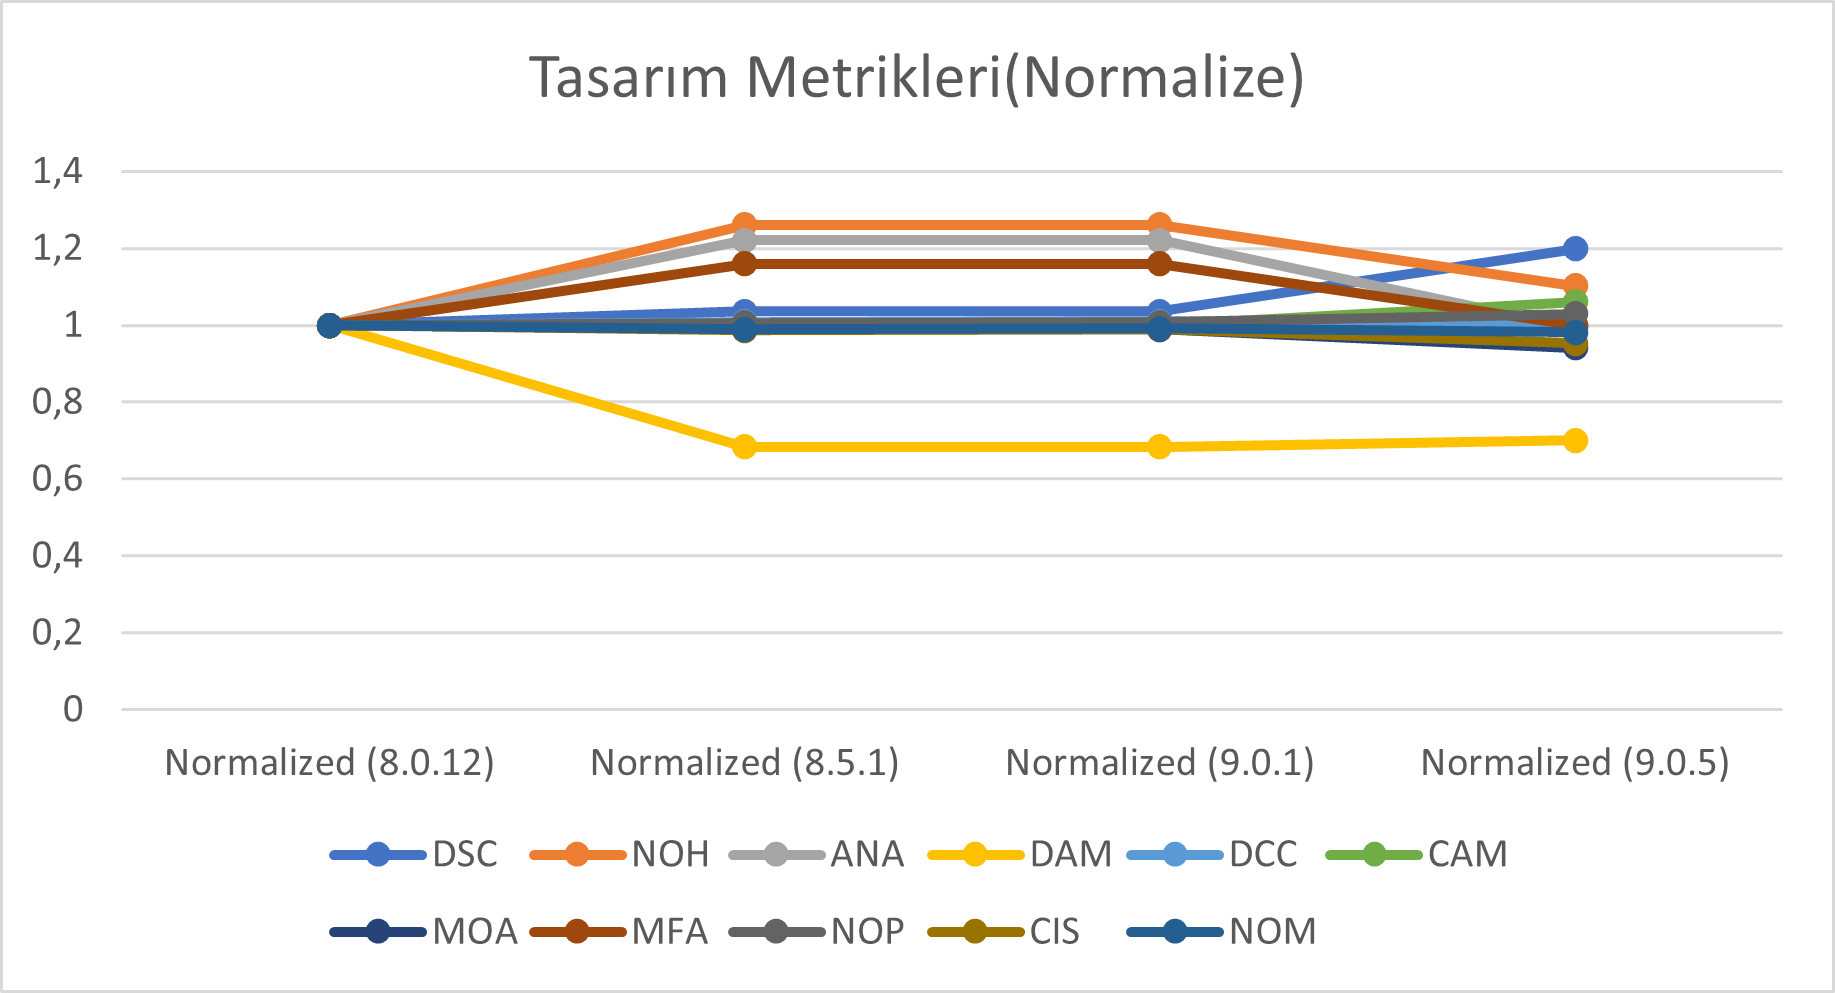
\includegraphics[scale=0.6]{metrik.png}
	\caption{Tasarım Metrikleri}
	\label{sekil1}
\end{figure}

\begin{figure}[h]
	\centering
	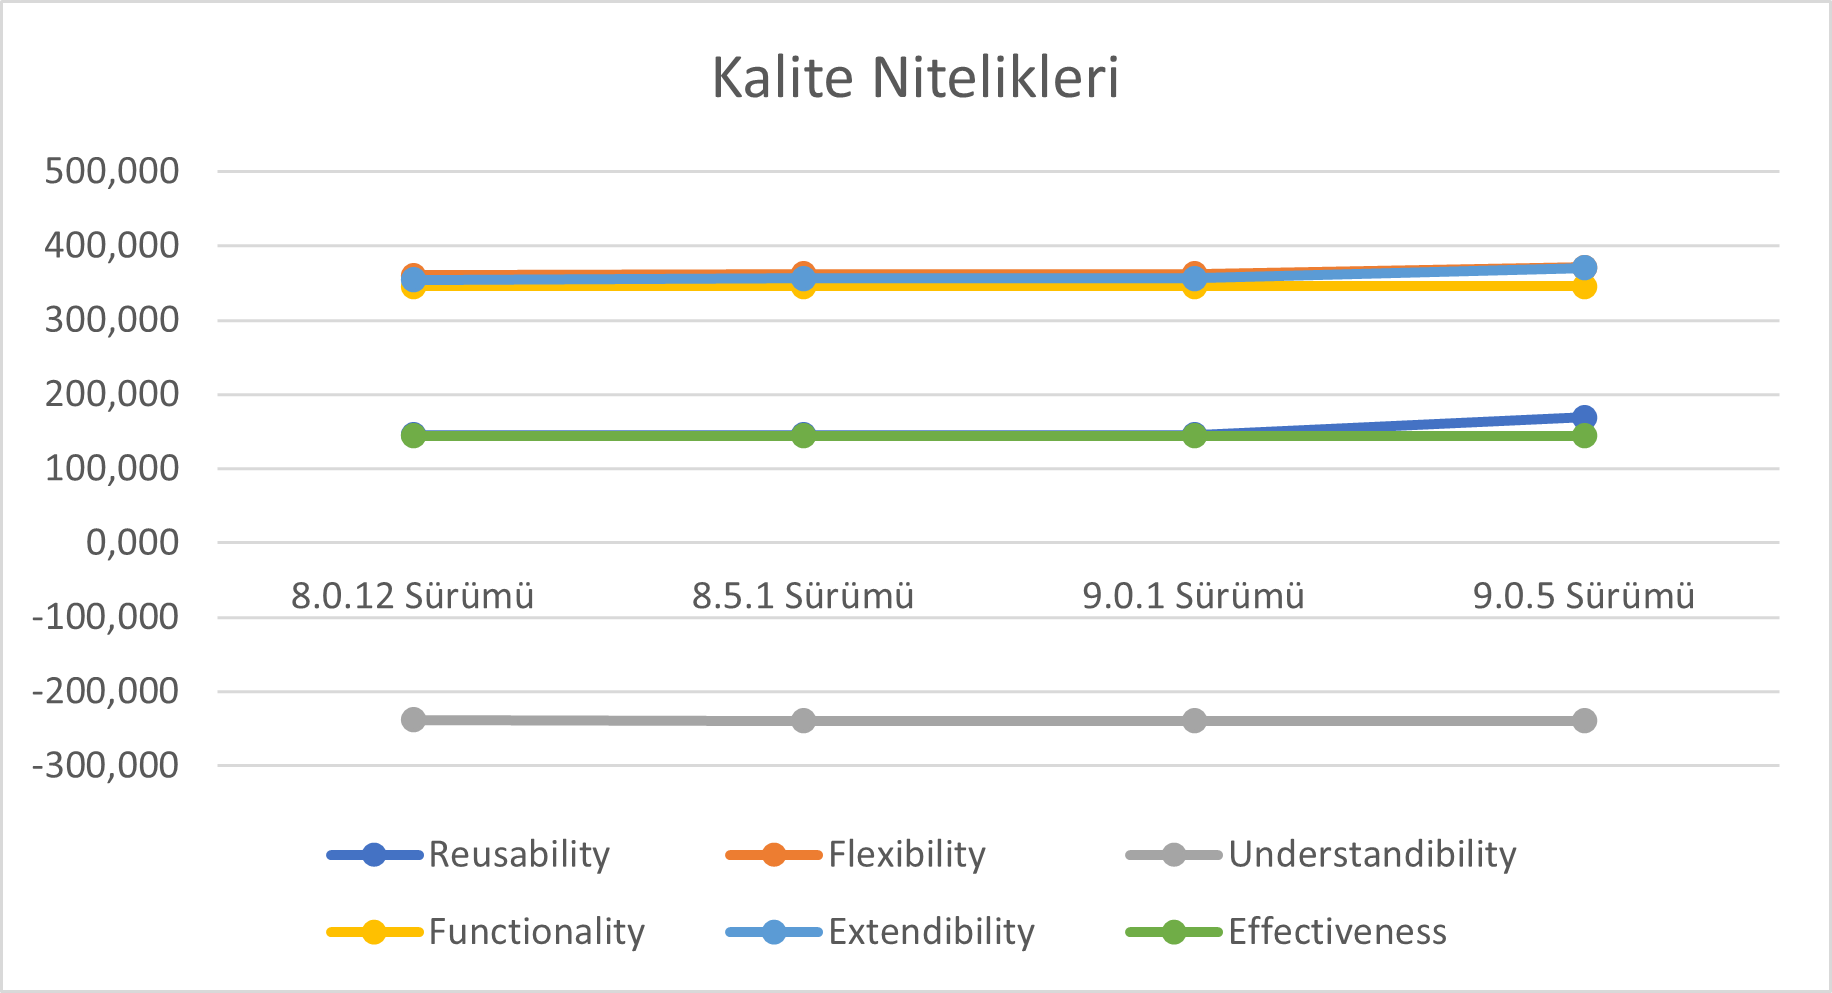
\includegraphics[scale=0.6]{nitelik.png}
	\caption{Kalite Nitelikleri}
	\label{sekil2}
\end{figure}

\begin{figure}[h]
	\centering
	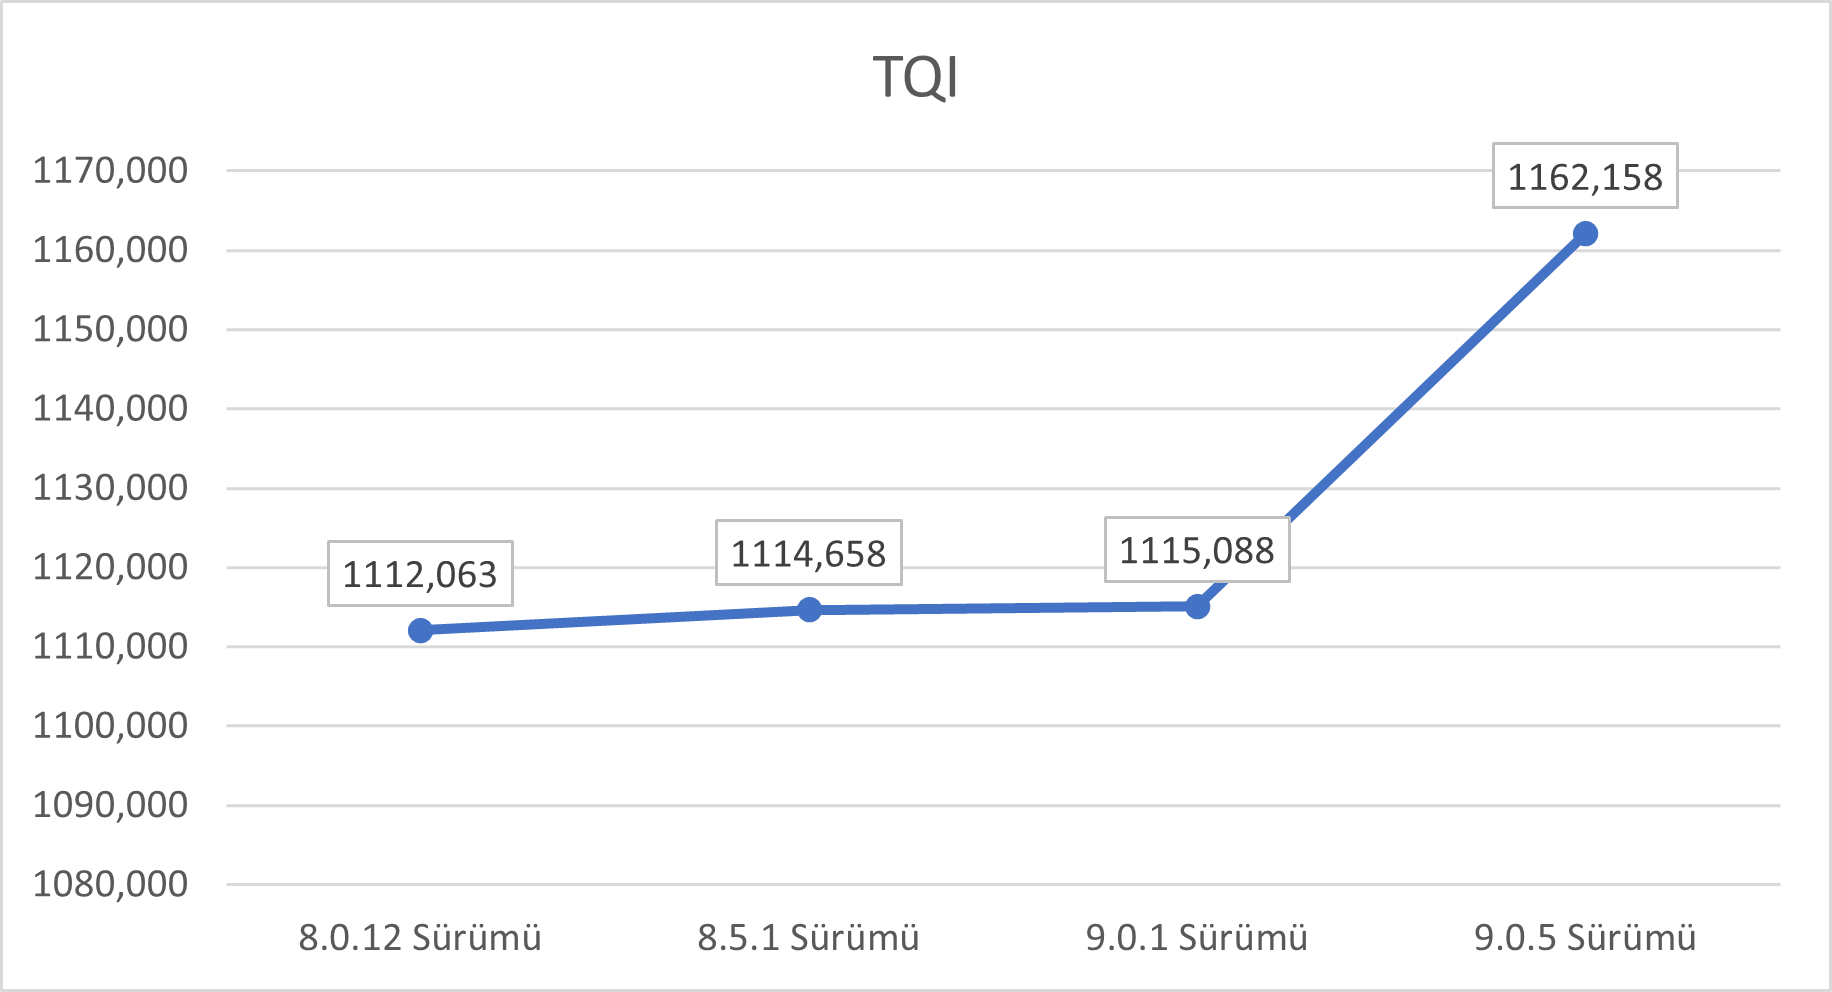
\includegraphics[scale=0.6]{tqi.png}
	\caption{TQI}
	\label{sekil3}
\end{figure}

\section{SONUÇ}

Bu çalışma, tasarım metrikleri ve tasarım özellikleri arasındaki ilişkileri derinlemesine inceleyerek, yazılım mühendisliği alanında önemli bir katkı sağlamıştır. Araştırmanın temel amacı, çeşitli tasarım özelliklerinin, yazılım kalitesi üzerindeki etkilerini nicel olarak değerlendirmekti. Bu amaç doğrultusunda, Design Size, Coupling, Cohesion gibi özellikler üzerinde yoğunlaşılmış ve bu özelliklerin yazılımın tekrar kullanılabilirliği, esnekliği, anlaşılabilirliği, işlevselliği, genişletilebilirliği ve etkinliği üzerindeki etkileri analiz edilmiştir.

Çalışmanın bulguları, yazılım tasarımının kalitesinin, belirli metrikler üzerinden ölçülebileceğini ve bu metriklerin yazılımın genel kalitesi üzerinde doğrudan etkileri olduğunu göstermektedir. Örneğin, Design Size ve Coupling metriklerinin, yazılımın tekrar kullanılabilirliği ve esnekliği üzerinde önemli etkileri tespit edilmiştir. Bu sonuçlar, yazılım tasarım süreçlerinin iyileştirilmesi ve daha kaliteli yazılım ürünlerinin geliştirilmesi konusunda önemli ipuçları sunmaktadır.

Bununla birlikte, çalışmanın kapsamındaki sınırlamalar da göz önünde bulundurulmalıdır. Araştırma, belirli bir yazılım türü ve ölçek üzerinde yapılmış olup, bulguların diğer yazılım türleri ve ölçekler üzerinde tekrar değerlendirilmesi gerekebilir. Ayrıca, tasarım metriklerinin farklı yazılım geliştirme ortamlarında nasıl değişkenlik gösterebileceği konusu, gelecekteki araştırmalar için önemli bir alan olarak belirlenmiştir.

Sonuç olarak, bu çalışma, yazılım mühendisliği alanında, tasarım kalitesini değerlendirmek ve geliştirmek için kullanılabilecek önemli metrikler ve ölçütler sunmaktadır. Elde edilen bulguların, yazılım geliştirme süreçlerinin daha etkin ve verimli hale getirilmesine katkıda bulunacağına inanılmaktadır. Gelecekteki çalışmaların, bu araştırmanın temelleri üzerine inşa edilerek, yazılım tasarım ve kalite değerlendirme metodolojilerini daha da ileriye taşıyacağı umulmaktadır.

\textbf{HATIRLATMA:} Metinde yer alan tüm formül, tablo, resim, referans vb. içerikleri en az 1 kez metin içerisinde atıflayınız.
Bu bir referans alıntısıdır: \cite{label}.

\begin{thebibliography}{1}
	
	\bibitem{bansiyadavis}
	J. Bansiya, C.G. Davis, "A hierarchical model for object-oriented design quality assessment", IEEE Transactions on Software Engineering, 28(1), 4-17, 2002.
	
	\bibitem{ozcevik}
	Y. Özçevik, "Simplified QMOOD Model Proposal Based on Correlation Analysis in Different Client Applications", 2021 29th Signal Processing and Communications Applications Conference (SIU), 1-4, 2021.
	
	\bibitem{mccall}
	McCall, J. A., Richards, P. K. and Walters, G. F., "Factors in Software Quality", Nat’l Tech.Information Service, no. Vol. 1, 2 and 3, (1977).
	
	\bibitem{basili}
	Victor R. Basili, Gianluigi Caldiera, H. Dieter Rombach, “The Goal Question Metric Approach”, Encyclopedia of Software Engineering, Wiley1994.
	
	\bibitem{isoiec9126}
	ISO “ISO,IEC 9126”,http://www.iso.org
	
\end{thebibliography}



\end{document}
